\RequirePackage[l2tabu, orthodox]{nag}

\documentclass{article}

\usepackage[margin=1.9cm, letterpaper]{geometry}
\usepackage[utf8]{inputenc}
\usepackage[a-1b]{pdfx}
\usepackage{indentfirst}
\usepackage{tikz}
\usepackage{float}
\usepackage{subcaption}
\usepackage{mathtools}
\usepackage{amssymb}
\usepackage{booktabs}
\usepackage{siunitx}
\usepackage{pdfpages}
\usepackage[outputdir=obj]{minted}
\usepackage{fontspec}
\usepackage{hyperref}
\usepackage[style=ieee]{biblatex}
\usepackage{karnaugh-map}

\setmainfont{Cambria}
\setsansfont{Segoe UI}
\setmonofont{Consolas}

\usemintedstyle{xcode}
\setminted{fontsize=\footnotesize, linenos=true, breaklines}

\begin{document}
\begin{titlepage}
    \begin{center}
        \vspace*{1cm}

        \textbf{\Large{LAB 1}}

        \vspace{0.5cm}

        \LARGE{Implementing Binary Adders in VHDL}

        \vspace{1.5cm}

        \textbf{\Large{Michael Kwok (1548454)}}

        \vfill

        ECE 410 -- Advanced Digital Logic Design\\
        Department of Electrical and Computer Engineering\\
        University of Alberta\\
        October 6, 2021

    \end{center}
\end{titlepage}

\tableofcontents
\listoffigures
\listoftables

\pagebreak

\section{Abstract}

In this report, an exploration of two different approaches to digital logic design was done: the register-transfer level and structural approach.
Two different implementations of a 2-bit full adder were designed, and the resource usage of each implementation was compared.
The VHDL feature of multiple architecture definitions was used to make testing and implementation easier,
as the specific version was selected in the top-level configuration,
avoiding commenting out code or modifying code before synthesis.
The results of this lab show that the RTL-based design is more efficient when compared to the MUX-based design for 2-bit adders.

\section{Design}

\subsection{RTL Design}

\begin{table}[H]
\centering
\begin{subfigure}{\linewidth}
    \centering
    \begin{tabular}{c c c | c c}
        \toprule
        $A$ & $B$ & $C_{in}$ & $Sum$ & $C_{out}$ \\
        \midrule
        0   & 0   & 0        & 0     & 0         \\
        0   & 0   & 1        & 1     & 0         \\
        0   & 1   & 0        & 1     & 0         \\
        0   & 1   & 1        & 0     & 1         \\
        1   & 0   & 0        & 1     & 0         \\
        1   & 0   & 1        & 0     & 1         \\
        1   & 1   & 0        & 0     & 1         \\
        1   & 1   & 1        & 1     & 1         \\
        \bottomrule
    \end{tabular}
    \caption{Truth Table for 1-bit full adder}
    \label{tab:truth-table-1b}
\end{subfigure}

\begin{subfigure}{0.4\linewidth}
\begin{karnaugh-map}[4][2][1][$AB$][$C_{in}$]
\minterms{1,2,4,7}
\autoterms[0]
\implicant{1}{1}
\implicant{2}{2}
\implicant{4}{4}
\implicant{7}{7}
\end{karnaugh-map}
\caption{Karnaugh Map for $F$}
\label{diag:kmap-f}
\end{subfigure}
\begin{subfigure}{0.4\linewidth}
\begin{karnaugh-map}[4][2][1][$AB$][$C_{in}$]
\minterms{3,5,6,7}
\autoterms[0]
\implicant{3}{7}
\implicant{5}{7}
\implicant{7}{6}
\end{karnaugh-map}
\caption{Karnaugh Map for $C_{out}$}
\label{diag:kmap-c}
\end{subfigure}
\caption{Truth tables for 1-bit full adder}
\end{table}

Initially, a truth table for a 1-bit full adder was made (Table~\ref{tab:truth-table-1b}).
Corresponding Karnaugh maps were subsequently constructed from the values (Figures~\ref{diag:kmap-f} \&~\ref{diag:kmap-c}).
As can be seen, $F$ can be constructed by simply getting the xor of the terms, $F = A \oplus B \oplus C$,
and $C_{out}$ can be constructed by minterm implicants: $C_{out} = AB + BC_{in} + AC_{in}$.
For a 2-bit adder, the previous expressions can be applied to each bit to form each corresponding output bit,
with the $C_{out}$ of the least significant bit connected to the $C_{in}$ of the most significant bit.

\begin{figure}[H]
    \centering
    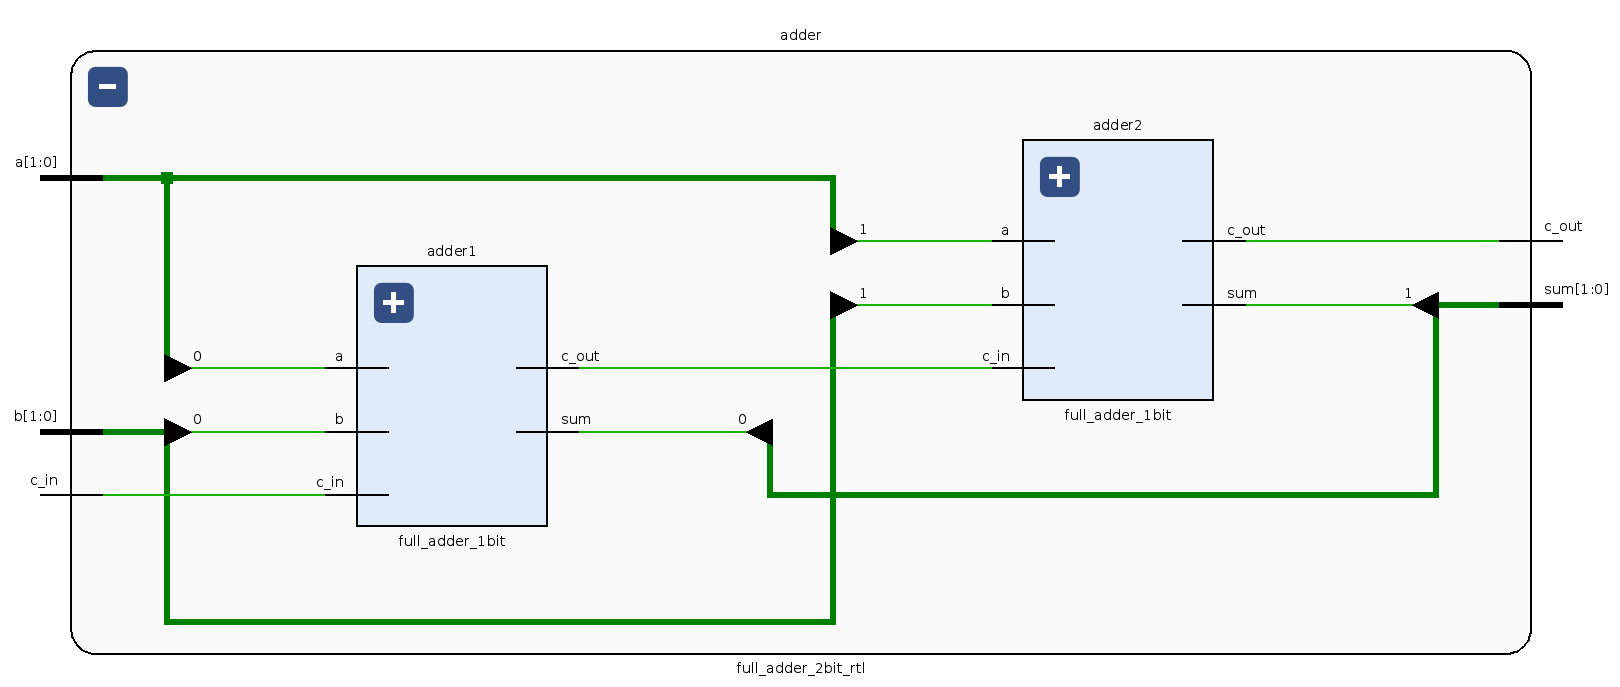
\includegraphics[width=0.53\textwidth]{rtl-schematic.png}
    \caption{Block Diagram of RTL design}
    \label{fig:rtl-schematic}
\end{figure}

This circuit was implemented at the RTL level in VHDL, as shown in the code in the appendix.
Two instances of the adder were chained together to form a ripple-carry 2-bit full adder,
which produced a circuit with three inputs and two outputs: two 2-bit vectors for the summands,
a 1-bit input for the carry-in, a 1-bit carry out and a 2-bit vector sum output.
The synthesized block diagram is shown in Figure~\ref{fig:rtl-schematic}.

\subsection{MUX Design}

A second version of the circuit was created, using three 16x1 MUXes to try out MUX-based circuit design.
Each MUX used the concatenated values of A and B as the selector.
The output was based on either short circuit to ground, VDD, $C_{in}$ or $\overline{C_{in}}$.

\begin{table}[H]
    \centering
    \begin{subfigure}{0.4\linewidth}
        \caption{Full table}
        \label{tab:truth-table-mux}
        \begin{tabular}{c c c | c c c}
            \toprule
            $A$ & $B$ & $C_{in}$ & $C_{out}$ & $S_1$ & $S_0$ \\
            \midrule
            00  & 00  & 0        & 0         & 0     & 0     \\
            00  & 00  & 1        & 0         & 0     & 1     \\
            00  & 01  & 0        & 0         & 0     & 1     \\
            00  & 01  & 1        & 0         & 1     & 0     \\
            00  & 10  & 0        & 0         & 1     & 0     \\
            00  & 10  & 1        & 0         & 1     & 1     \\
            00  & 11  & 0        & 0         & 1     & 1     \\
            00  & 11  & 1        & 1         & 0     & 0     \\
            01  & 00  & 0        & 0         & 0     & 1     \\
            01  & 00  & 1        & 0         & 1     & 0     \\
            01  & 01  & 0        & 0         & 1     & 0     \\
            01  & 01  & 1        & 0         & 1     & 1     \\
            01  & 10  & 0        & 0         & 1     & 1     \\
            01  & 10  & 1        & 1         & 0     & 0     \\
            01  & 11  & 0        & 1         & 0     & 0     \\
            01  & 11  & 1        & 1         & 0     & 1     \\
            10  & 00  & 0        & 0         & 1     & 0     \\
            10  & 00  & 1        & 0         & 1     & 1     \\
            10  & 01  & 0        & 0         & 1     & 1     \\
            10  & 01  & 1        & 1         & 0     & 0     \\
            10  & 10  & 0        & 1         & 0     & 0     \\
            10  & 10  & 1        & 1         & 0     & 1     \\
            10  & 11  & 0        & 1         & 0     & 1     \\
            10  & 11  & 1        & 1         & 1     & 0     \\
            11  & 00  & 0        & 0         & 1     & 1     \\
            11  & 00  & 1        & 1         & 0     & 0     \\
            11  & 01  & 0        & 1         & 0     & 0     \\
            11  & 01  & 1        & 1         & 0     & 1     \\
            11  & 10  & 0        & 1         & 0     & 1     \\
            11  & 10  & 1        & 1         & 1     & 0     \\
            11  & 11  & 0        & 1         & 1     & 0     \\
            11  & 11  & 1        & 1         & 1     & 1     \\
            \bottomrule
        \end{tabular}
    \end{subfigure}
    \begin{subfigure}{0.4\linewidth}
        \caption{Simplified for MUX}
        \label{tab:mux-simplified}
        \begin{tabular}{c c | c c c}
            \toprule
            $A$ & $B$ & $C_{out}$ & $S_1$               & $S_0$               \\
            \midrule
            00  & 00  & 0         & 0                   & $C_{in}$            \\
            00  & 01  & 0         & $C_{in}$            & $\overline{C_{in}}$ \\
            00  & 10  & 0         & 1                   & $C_{in}$            \\
            00  & 11  & $C_{in}$  & $\overline{C_{in}}$ & $\overline{C_{in}}$ \\
            01  & 00  & 0         & $C_{in}$            & $\overline{C_{in}}$ \\
            01  & 01  & 0         & 1                   & $C_{in}$            \\
            01  & 10  & $C_{in}$  & $\overline{C_{in}}$ & $\overline{C_{in}}$ \\
            01  & 11  & 0         & 0                   & $C_{in}$            \\
            10  & 00  & 0         & 1                   & $C_{in}$            \\
            10  & 01  & $C_{in}$  & $\overline{C_{in}}$ & $\overline{C_{in}}$ \\
            10  & 10  & 0         & 0                   & $C_{in}$            \\
            10  & 11  & 0         & $C_{in}$            & $\overline{C_{in}}$ \\
            11  & 00  & $C_{in}$  & $\overline{C_{in}}$ & $\overline{C_{in}}$ \\
            11  & 01  & 0         & 0                   & $C_{in}$            \\
            11  & 10  & 0         & $C_{in}$            & $\overline{C_{in}}$ \\
            11  & 11  & 0         & 1                   & $C_{in}$            \\
            \bottomrule
        \end{tabular}
    \end{subfigure}
    \caption{Truth tables for 2-bit full adder}
\end{table}

\begin{figure}[h]
    \centering
    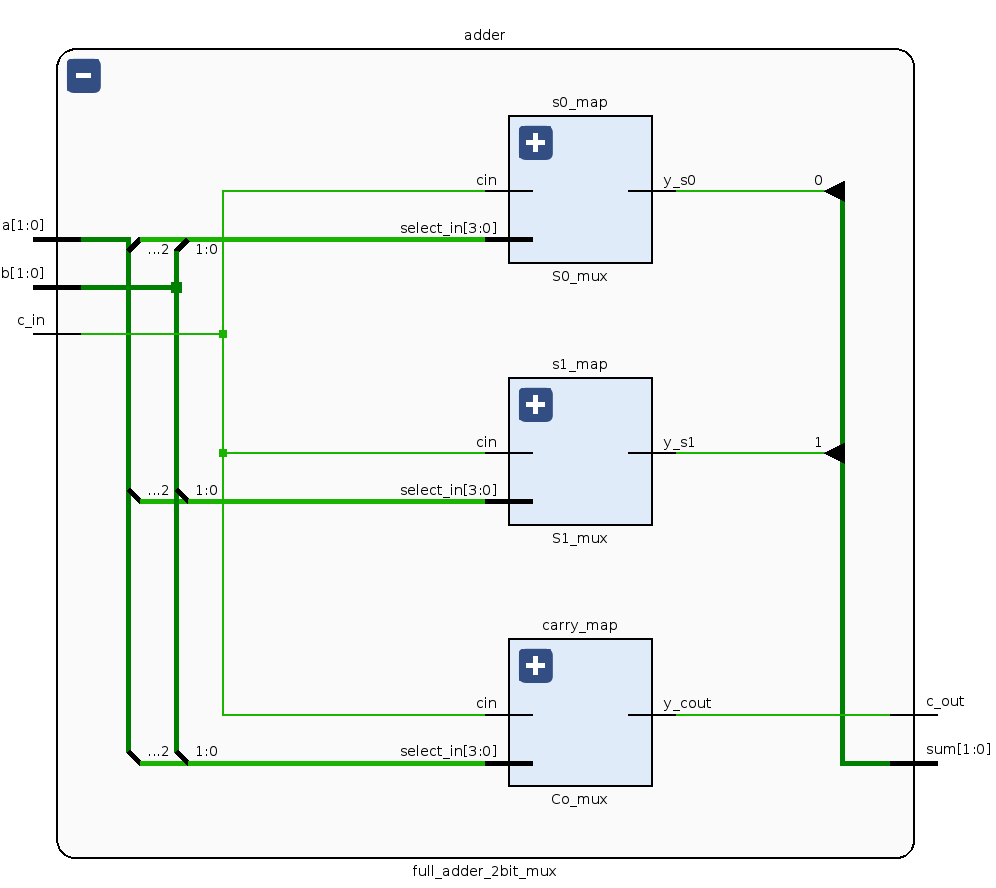
\includegraphics[width=0.5\linewidth]{mux-schematic.png}
    \caption{Block Diagram of MUX design}
    \label{fig:mux-schematic}
\end{figure}

As part of this process, a 32 entry truth table was constructed (Table~\ref{tab:truth-table-mux}).
This was extremely time consuming and error prone, as the work was ``monotonous'', and it quickly became hard to keep track
of the binary numbers that were being written. While a Karnaugh Map was not required,
the values for $C_{out}$, $S_1$ and $S_0$ had to be simplified by hand to and redefined in terms of $C_{in}$ for each MUX input.
The result of simplification is shown in Table~\ref{tab:mux-simplified}.
This all resulted in the synthesis of 3 MUXes for the circuit (Figure~\ref{fig:mux-schematic}), as expected.

\subsection{Comparator}

For the comparator, a behavioural implementation was done. This was to allow the synthesis and implementation tools to
optimize the design as best as possible by providing it with semantically as much information as possible.

The schematic generated by the tool can be seen in Figure~\ref{fig:comp-schematic}.

\begin{figure}[h]
    \centering
    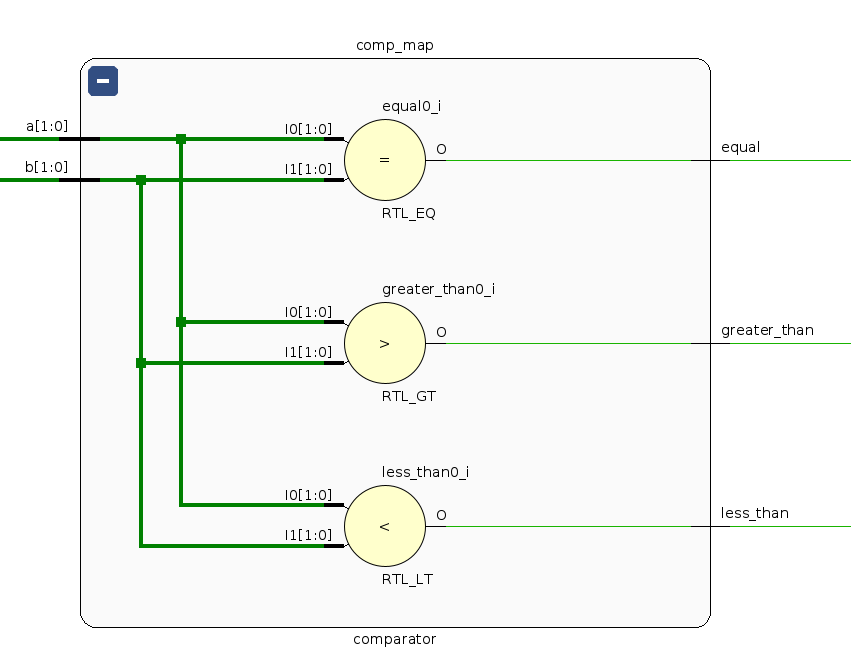
\includegraphics[width=0.6\linewidth]{comp-schematic.png}
    \caption{Block Diagram of Comparator design}
    \label{fig:comp-schematic}
\end{figure}

\pagebreak

\subsection{FPGA Implementation}

In terms of implementation, the MUX design produced a less efficient circuit resource utilization-wise,
with 3 LUTs required to implement the adder as compared to 2 for RTL.\@
A possible explanation for this could be that each 1-bit full adder was implemented as a LUT for the RTL Design,
instead of a single LUT for each output bit for the MUX Design.

\begin{figure}[h]
    \centering
    \begin{subfigure}{0.45\linewidth}
        \centering
        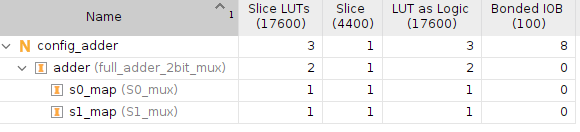
\includegraphics[width=\textwidth]{mux-resource.png}
        \caption{MUX Design}
    \end{subfigure}
    \begin{subfigure}{0.45\linewidth}
        \centering
        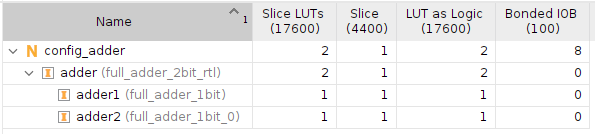
\includegraphics[width=\textwidth]{rtl-resource.png}
        \caption{RTL Design}
    \end{subfigure}
    \caption{Resource utilization of both designs}
    \label{fig:resource}
\end{figure}

The MUX design might be faster than the RTL design since there is no need to wait for the result of the addition of the first bit,
and the entire 2-bit output is produced at the same time. In order to prove this, timing analysis must be done,
which is unnecessary for a 2-bit adder as any delay due to ripple carry is likely to be below the margin of error.

\section{Testing \& Simulation}

\begin{figure}[h]
    \centering
    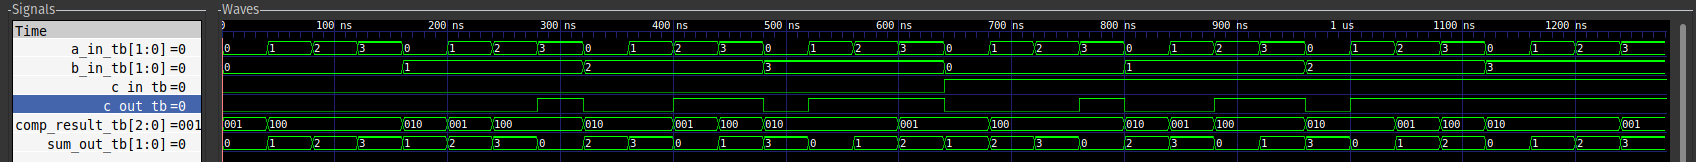
\includegraphics[width=\linewidth]{tb-result.png}
    \caption{Waveform Screenshot}
    \label{fig:tb-result}
\end{figure}

For the testing and simulation of the components, a testbench was written and ran for both implementations of the device.
The resulting waveforms were compared to ensure proper operation of the design, and the waveform can be seen in Figure~\ref{fig:tb-result}.

The designed testbench was written to loop through all possible values of $A$, $B$ and $C_{in}$.
As shown, the adders worked as expected.

The designs were tested on the Zybo board provided, and the expected results were obtained by manipulating the buttons and switches on the board.

\section{Conclusion}

In this lab we have shown two different methods of obtaining the same result, with each having their own advantages and disadvantages.
The RTL method of defining the circuit led to shorter and easier to understand code, while the MUX method is potentially faster if
extended to more than 2-bit addition, since it's an implicit ``carry-lookahead'' adder.
The difference in resource utilization was also shown, with the RTL implementation leading by using less resources than the MUX.\@
The comparator implementation shows that behavioural VHDL can be simpler and as effecient as RTL or Structural VHDL.\@

The importance of writing extensive testbenches was made apparent, as it helped caught a lot of possible errors in the
implementation of the MUX by stopping whenever there was an error, allowing iterative improvement and fixing.
Modularity of the MUX design also helped with debugging as each bit had a corresponding module, so it was very easy to track where the issue was.

% \section{References}

\pagebreak
\section*{Appendix}

\subsection{Top Level File}
\inputminted{vhdl}{../src/lab1_top.vhd}

\pagebreak
\subsection{1-bit full adder}
\inputminted{vhdl}{../src/full_adder_1bit.vhd}

\pagebreak
\subsection{2-bit full adder}
\inputminted{vhdl}{../src/full_adder_2bit.vhd}

\pagebreak
\subsection{Cout MUX}
\inputminted{vhdl}{../src/Co_mux.vhd}

\pagebreak
\subsection{S1 MUX}
\inputminted{vhdl}{../src/S1_mux.vhd}

\pagebreak
\subsection{S0 MUX}
\inputminted{vhdl}{../src/S0_mux.vhd}

\pagebreak
\subsection{Comparator}
\inputminted{vhdl}{../src/Comparator.vhd}

\pagebreak
\subsection{Testbench}
\inputminted{vhdl}{../test/full_adder_2bit_tb.vhd}

\renewcommand{\thepage}{}

\end{document}
